%convert -coalesce launch.gif launch_%d.png
\documentclass{beamer}

\newcommand{\VEV}[1]{\langle#1\rangle}
\newcommand{\sst}{\left(1-\frac{2M}{r}\right)}
\newcommand{\sh}{\mathrm{shell}}
\newcommand{\be}{\begin{equation}}
\newcommand{\ee}{\end{equation}}
\newcommand{\bue}{\begin{equation}}
\newcommand{\eue}{\end{equation}}
\newcommand{\bc}{\begin{center}}
\newcommand{\ec}{\end{center}}
\newcommand{\bea}[1]{\begin{eqnarray}\label{#1}}
\newcommand{\eea}{\end{eqnarray}}
\newcommand{\bua}{\begin{eqnarray*}}
\newcommand{\eua}{\end{eqnarray*}}
\newcommand{\dd}[2]{{{d#1}\over{d#2}}}
\newcommand{\ddt}[1]{\dd{#1}{t}}
\newcommand{\dddt}[1]{\dd{^2#1}{t^2}}
\newcommand{\aver}[1]{\langle{#1}\rangle}
\newcommand{\atom}[3]{\ifmmode^{#1}_{#2}{\rm{#3}}\else{$^{#1}_{#2}${#3}}\fi}
\newcommand{\electron}{\atom{~0}{-1}{e}}
\newcommand{\positron}{\atom{0}{0}{\bar{e}}}
\newcommand{\neutrino}{\atom{0}{0}{\nu_e}}
\newcommand{\photon}{\atom{0}{0}{\gamma}}
\newcommand{\antineutrino}{\atom{0}{0}{\bar{\nu}}}
\newcommand{\neutron}{\atom{1}{0}{n}}
\newcommand{\proton}{\atom{1}{1}{p}}
\newcommand{\hydrogen}{\atom{1}{1}{H}}
\newcommand{\deuterium}{\atom{2}{1}{H}}
\newcommand{\tritium}{\atom{3}{1}{H}}
\newcommand{\helium}{\atom{4}{2}{He}}
\newcommand{\hethree}{\atom{3}{2}{He}}

\renewcommand{\ss}{Schwarz\-schild }

\def\densu{kg/m$^3$} 
\def\rsol{R$_{\odot}$} 
\def\msol{M$_{\odot}$} 

\newcommand{\htmlcom}[1]{}


\usetheme{Boadilla}
%\usepackage{multimedia}
%\usepackage{animate}
\usepackage{hyperref}
\usepackage{tikz}
\usepackage{cancel}
\usepackage{tikzsymbols}
\usepackage{ifthen}

%%%%mathcircled
\makeatletter
\newcommand\mathcircled[1]{%`
  \mathpalette\@mathcircled{#1}%
}
\newcommand\@mathcircled[2]{%
  \tikz[baseline=(math.base)] \node[draw,circle,red, thick, inner sep=2pt] (math) {$\m@th#1#2$};%
}
\makeatother
%%%%

%gets rid of bottom navigation bars
\setbeamertemplate{footline}[frame number]{} %begin

%gets rid of bottom navigation symbols
\setbeamertemplate{navigation symbols}{}

%gets rid of footer
%will override 'frame number' instruction above  %begin
%comment out to revert to previous/default definitions
\setbeamertemplate{footline}{}

\definecolor{darkscarlet}{rgb}{0.34, 0.01, 0.1}
\definecolor{gold(metallic)}{rgb}{0.83, 0.69, 0.22}
\definecolor{green(ryb)}{rgb}{0.4, 0.69, 0.2}
\definecolor{darkorange}{rgb}{1.0, 0.55, 0.0}
\definecolor{amber}{rgb}{1.0, 0.75, 0.0}
\definecolor{bronze}{rgb}{0.8, 0.5, 0.2}
\definecolor{cadet}{rgb}{0.33, 0.41, 0.47}
\definecolor{silver}{rgb}{0.75, 0.75, 0.75}
\definecolor{turquoise}{rgb}{0.19, 0.84, 0.78}
\definecolor{uclagold}{rgb}{1.0, 0.7, 0.0}
\definecolor{urobilin}{rgb}{0.88, 0.68, 0.13}
\definecolor{vegasgold}{rgb}{0.77, 0.7, 0.35}
\definecolor{vanilla}{rgb}{0.95, 0.9, 0.67}
\definecolor{straw}{rgb}{0.89, 0.85, 0.44}
\definecolor{sunset}{rgb}{0.98, 0.84, 0.65}
\definecolor{brown(traditional)}{rgb}{0.59, 0.29, 0.0}
\definecolor{apricot}{rgb}{0.98, 0.81, 0.69}
\definecolor{darkblue}{rgb}{0,0,0.54}

\hypersetup{
    colorlinks=true,
    linkcolor=yellow,
    filecolor=magenta,
    urlcolor=blue,
}

\let\hrefori\href
\renewcommand{\href}[2]{{\setlength{\fboxsep}{1pt}\colorbox{sunset}{\hrefori{#1}{#2}}}}


%title
\setbeamercolor{block title alerted}{fg=white,bg=cyan}
%body
\setbeamercolor{block body alerted}{fg=black!90,bg=yellow!60}

%title
\setbeamercolor{block title}{fg=black,bg=turquoise}
%body
\setbeamercolor{block body}{fg=yellow,bg=bronze}




\newcommand{\pagebutton}[1]{\setbeamertemplate{button}{\tikz\node[inner xsep = 5pt, draw = structure!90, fill = green(ryb), rounded corners = 8pt]{\color{amber}\Large\insertbuttontext};}\beamerbutton{#1}}

\newcommand{\choicebutton}[1]{\setbeamertemplate{button}{\tikz\node[inner xsep = 8pt, draw = structure!90, fill = vegasgold, rounded corners = 5pt]{\color{vanilla}\Large\insertbuttontext};}\beamerbutton{#1}}

\newcommand{\pagenobutton}[1]{\setbeamertemplate{button}{\tikz\node[inner xsep = 8pt, draw = structure!90, fill = apricot, rounded corners = 5pt]{\color{brown(traditional)}\Large\insertbuttontext};}\beamerbutton{#1}}

\newcommand{\headlinebutton}[1]{\setbeamertemplate{button}{\tikz\node[inner xsep = 8pt, draw = structure!90, fill = blue, rounded corners = 5pt]{\color{yellow}\Large\insertbuttontext};}\beamerbutton{#1}}

\newcommand{\forumbutton}{\href{https://astro-discourse.utenforuio.no/c/ast2000/sporsmal-til-forelesningsnotatene-del-3a-3e/18}{\setbeamertemplate{button}{\tikz\node[inner xsep = 8pt, draw = structure!90, fill = darkblue, rounded corners = 5pt]{\color{yellow}\Large\insertbuttontext};}\beamerbutton{\textcolor{red}{\small FORUM}}}}

\newcommand{\curpage}{\pagenobutton{\small side \thepageno\  av \thenopages}}
\newcommand{\nextpage}{\refstepcounter{pageno}\pagenobutton{\small side \thepageno\  av \thenopages}}
\newcommand{\dnextpage}{\refstepcounter{pageno}\refstepcounter{pageno}\pagenobutton{\small side \thepageno\  av \thenopages}}

\newcommand{\lastpagebutton}[1]{\hyperlink{#1}{\pagebutton{\small Forrige side}}\href{https://nettskjema.no/a/167471}{\Changey[1][yellow]{2} \Changey[1][yellow]{-2}}\nextpage\headlinebutton{\headline}\forumbutton}
\newcommand{\clastpagebutton}[1]{\hyperlink{#1}{\pagebutton{\small Forrige side}}\href{https://nettskjema.no/a/167471}{\Changey[1][yellow]{2} \Changey[1][yellow]{-2}}\curpage\headlinebutton{\headline}\forumbutton}
\newcommand{\dlastpagebutton}[1]{\hyperlink{#1}{\pagebutton{\small Forrige side}}\href{https://nettskjema.no/a/167471}{\Changey[1][yellow]{2} \Changey[1][yellow]{-2}}\dnextpage\headlinebutton{\headline}\forumbutton}

\newcommand{\lastpagebuttonx}[1]{\hyperlink{#1}{\pagebutton{\small Forrige side}}\href{https://nettskjema.no/a/167471}{\Changey[1][yellow]{2} \Changey[1][yellow]{-2}}\nextpage\\}
\newcommand{\clastpagebuttonx}[1]{\hyperlink{#1}{\pagebutton{\small Forrige side}}\href{https://nettskjema.no/a/167471}{\Changey[1][yellow]{2} \Changey[1][yellow]{-2}}\curpage\\}
\newcommand{\dlastpagebuttonx}[1]{\hyperlink{#1}{\pagebutton{\small Forrige side}}\href{https://nettskjema.no/a/167471}{\Changey[1][yellow]{2} \Changey[1][yellow]{-2}}\dnextpage\\}

\newcommand{\lastpagebuttoncr}[1]{\hyperlink{#1}{\pagebutton{\small Forrige side}}\href{https://nettskjema.no/a/167471}{\Changey[1][yellow]{2} \Changey[1][yellow]{-2}}\nextpage\\\headlinebutton{\headline}\forumbutton\\}
\newcommand{\clastpagebuttoncr}[1]{\hyperlink{#1}{\pagebutton{\small Forrige side}}\href{https://nettskjema.no/a/167471}{\Changey[1][yellow]{2} \Changey[1][yellow]{-2}}\curpage\\\headlinebutton{\headline}\forumbutton\\}
\newcommand{\dlastpagebuttoncr}[1]{\hyperlink{#1}{\pagebutton{\small Forrige side}}\href{https://nettskjema.no/a/167471}{\Changey[1][yellow]{2} \Changey[1][yellow]{-2}}\dnextpage\\\headlinebutton{\headline}\forumbutton\\}

\newcommand{\nytemaside}[1]{
\centerline{\Huge\textcolor{yellow}{Nytt tema:}}\\
\vspace*{1cm}
\centerline{\Large\bf\textcolor{yellow}{\headline}}
\vspace*{2cm}
\ifthenelse{\equal{#1}{0}}{\centerline{\textcolor{yellow}{Siste tema i denne forelesningen!}}}{\centerline{\textcolor{yellow}{\footnotesize Dette temaet fortsetter frem til side \ref{#1} av \thenopages.}}}
\vspace*{0.5cm}
}


\newcommand{\fullframe}[6]{
\begin{frame}
\label{#1}
\addtocounter{pageno}{#4}
\lastpagebutton{#2}{\bf #6}\\
#5
\hyperlink{#3}{\pagebutton{Neste side}}
\end{frame}
}



\newcommand{\fullframetwo}[7]{
\begin{frame}
\label{#1}
\addtocounter{pageno}{#4}
\lastpagebutton{#2}{\bf #7}\\
\begin{columns}
\column{0.5\textwidth}
#5
\column{0.5\textwidth}
#6
\hyperlink{#3}{\pagebutton{Neste side}}
\end{columns}
\end{frame}
}

\newcommand{\fullframetwonotxt}[7]{
\begin{frame}
\label{#1}
\addtocounter{pageno}{#4}
\lastpagebutton{#2}{\bf #7}\\
\begin{columns}
\column{0.5\textwidth}
#5
\column{0.5\textwidth}
#6
\end{columns}
\end{frame}
}



\newcommand{\fullframetxt}[7]{
\begin{frame}
\label{#1}
\addtocounter{pageno}{#4}
\lastpagebutton{#2}{\bf #7}\\
#6
\hyperlink{#3}{\pagebutton{#5}}
\end{frame}
}

\newcommand{\fullframenotxt}[6]{
\begin{frame}
\label{#1}
\addtocounter{pageno}{#4}
\lastpagebutton{#2}{\bf #6}\\
#5
\end{frame}
}

\newcommand{\choiceframe}[5]{
\begin{frame}
\label{#1}
\addtocounter{pageno}{#3}
\lastpagebutton{#2}{\bf #5}\\
#4
\end{frame}
}

\newcommand{\colfullframe}[7]{
{
\setbeamercolor{background canvas}{bg=#5}
\begin{frame}
\label{#1}
\addtocounter{pageno}{#4}
\lastpagebutton{#2}{\bf #7}\\
#6
\hyperlink{#3}{\pagebutton{Neste side}}
\end{frame}
}
}

\newcommand{\colfullframenotxt}[7]{
{
\setbeamercolor{background canvas}{bg=#5}
\begin{frame}
\label{#1}
\addtocounter{pageno}{#4}
\lastpagebutton{#2}{\bf #7}\\
#6
\end{frame}
}
}

\newcommand{\colfullframetwo}[8]{
{
\setbeamercolor{background canvas}{bg=#5}
\begin{frame}
\label{#1}
\addtocounter{pageno}{#4}
\lastpagebutton{#2}{\bf #8}\\
\begin{columns}
\column{0.5\textwidth}
#6
\column{0.5\textwidth}
#7
\hyperlink{#3}{\pagebutton{Neste side}}
\end{columns}
\end{frame}
}
}

\newcommand{\colfullframetwonotxt}[8]{
{
\setbeamercolor{background canvas}{bg=#5}
\begin{frame}
\label{#1}
\addtocounter{pageno}{#4}
\lastpagebutton{#2}{\bf #8}\\
\begin{columns}
\column{0.5\textwidth}
#6
\column{0.5\textwidth}
#7
\end{columns}
\end{frame}
}
}

\newcommand{\colfullframetxt}[8]{
{
\setbeamercolor{background canvas}{bg=#5}
\begin{frame}
\label{#1}
\addtocounter{pageno}{#4}
\lastpagebutton{#2}{\bf #8}\\
#7
\hyperlink{#3}{\pagebutton{#6}}
\end{frame}
}
}

\newcommand{\colchoiceframe}[6]{
{
\setbeamercolor{background canvas}{bg=#4}
\begin{frame}
\label{#1}
\addtocounter{pageno}{#3}
\lastpagebutton{#2}{\bf #6}\\
#5
\end{frame}
}
}


\newcommand{\pagequestion}[3]{
\hyperlink{#1}{\pagebutton{#2}}
\pause
%#3 normalt -1 for første spørsmål
\addtocounter{pageno}{#3}
\begin{itemize}[<+->]
\item[] \hypertarget<.>{#1}{}
\end{itemize}
\vspace{-0.5cm}
}

\newcommand{\samepagequestion}[4]{
\hyperlink{#1}{\pagebutton{#2}}\hyperlink{#1}{\pagebutton{#3}}
\pause
%#3 normalt -1 for første spørsmål
\addtocounter{pageno}{#4}
\begin{itemize}[<+->]
\item[] \hypertarget<.>{#1}{}
\end{itemize}
\vspace{-0.5cm}
}

\newcommand{\twopagequestion}[7]{
\hyperlink{#1}{\pagebutton{#3}}\hyperlink{#2}{\pagebutton{#4}}
\pause
%#3 normalt -1 for første spørsmål
\addtocounter{pageno}{#5}
\begin{itemize}[<+->]
\item[] \hypertarget<.>{#1}{}
\end{itemize}
\vspace{-0.5cm}
#7
\addtocounter{pageno}{#6}
\begin{itemize}[<+->]
\item[] \hypertarget<.>{#1}{}
\end{itemize}
\vspace{-0.5cm}
}

\newcounter{pageno}
\newcounter{nopages}
\setcounter{nopages}{42}

\newcommand{\headline}{\small Introduksjon}
\newcommand{\m}{\mathrm{m}}

\begin{document}

\begin{frame}
\label{front2}
\center{\Large \textcolor{darkscarlet}{\bf AST2000 Del 3D\\Interaktive forelesningsnotater: forelesning 2 av 2}}\\
\begin{block}{\center{\bf VIKTIG}}
\textcolor{yellow}{Dette er et alternativ til forelesningen i emnet.} \textcolor{blue}{Har du gått skikkelig gjennom disse interaktive forelesningsnotatene så trenger du ikke å lese \href{https://www.uio.no/studier/emner/matnat/astro/AST2000/h21/undervisningsmateriell/lecture_notes/part3d.pdf}{de fulle forelesningsnotatene} (med unntak av oppgavene bak)}. All informasjonen du trenger, får du her. Du kommer til å få mange grublespørsmål og diskusjonsoppgaver, det er meningen at disse skal gjøres i grupper av minst 2, maks 4 studenter. {\bf Det er defor sterkt anbefalt at dere sitter sammen i grupper når dere går gjennom disse interaktive forelesningsnotatene, du vil få betydelig mer utbytte av dem på den måten}. {\bf Hvis du har kommentarer ris/ros til disse forelesningsnotatene eller til emnet, trykk på \href{https://nettskjema.no/a/167471}{\Changey[1][yellow]{2} \Changey[1][yellow]{-2}}\ knappen som du finner på alle sider.}
\end{block}
%\setbeamercolor{button}{bg=black,fg=yellow}
\hyperlink{front3}{\pagebutton{Trykk denne knappen for å begynne}}
\end{frame}

\begin{frame}
\label{front3}
{\Large
\begin{itemize}
\item HUSK at du får mer ut av de interaktive forelesningsnotatene når du gjør de sammen med noen. Diskusjonene med andre er svært viktige.
\item Det er mange spørsmål/grubliser underveis, sett dere selv en tidsgrense, 1 minutt på de korte, maks 4-5 minutter på de lenger. Ha en alarm ved siden av, ellers kommer dere til å bruke alt for langt tid. Har dere ikke fått det til etter kort tid, gå videre, se svaret og lær!
\item Er du i det minste tvil om noe, så finnes det en \forumbutton knapp, trykk det og still spørsmål med en gang mens du enda husker spørsmålet!
\end{itemize}
}
\hyperlink{tableofcontents}{\pagebutton{Trykk denne knappen for å begynne}}
\end{frame}

\begin{frame}
\label{tableofcontents}
\hyperlink{front3}{\pagebutton{Forrige side}}\\
Hvis du allerede har begynt på denne forelesningen og vil hoppe rett inn til et annet kapittel, kan du trykke her:
\begin{itemize}
\item \hyperlink{blue_nytema1}{\headlinebutton{Levetid på hovedserien}}
\item \hyperlink{pause}{\headlinebutton{Kaffepausen}}
\item \hyperlink{ms26}{\headlinebutton{Hovedserien: oppsummering og tolkning}}
\item \hyperlink{blue_nytema2}{\headlinebutton{Farvel hovedserie!}}
\end{itemize}
Merk at sidene er merket med sidenummer på denne måten: SIDE X/Y/Z. Her er Z antall sider totalt, Y er sidenummeret til siste side i avsnittet du holder på med og X er sidenummeret til siden du er på.\\
\hyperlink{feil_intro}{\choicebutton{Neste side}}
\end{frame}

%%%%% intro
{
\setbeamercolor{background canvas}{bg=black}
\begin{frame}
\label{feil_intro}
\begin{columns}
\column{0.5\textwidth}
\hyperlink{front3}{\pagebutton{Forrige side}}\\
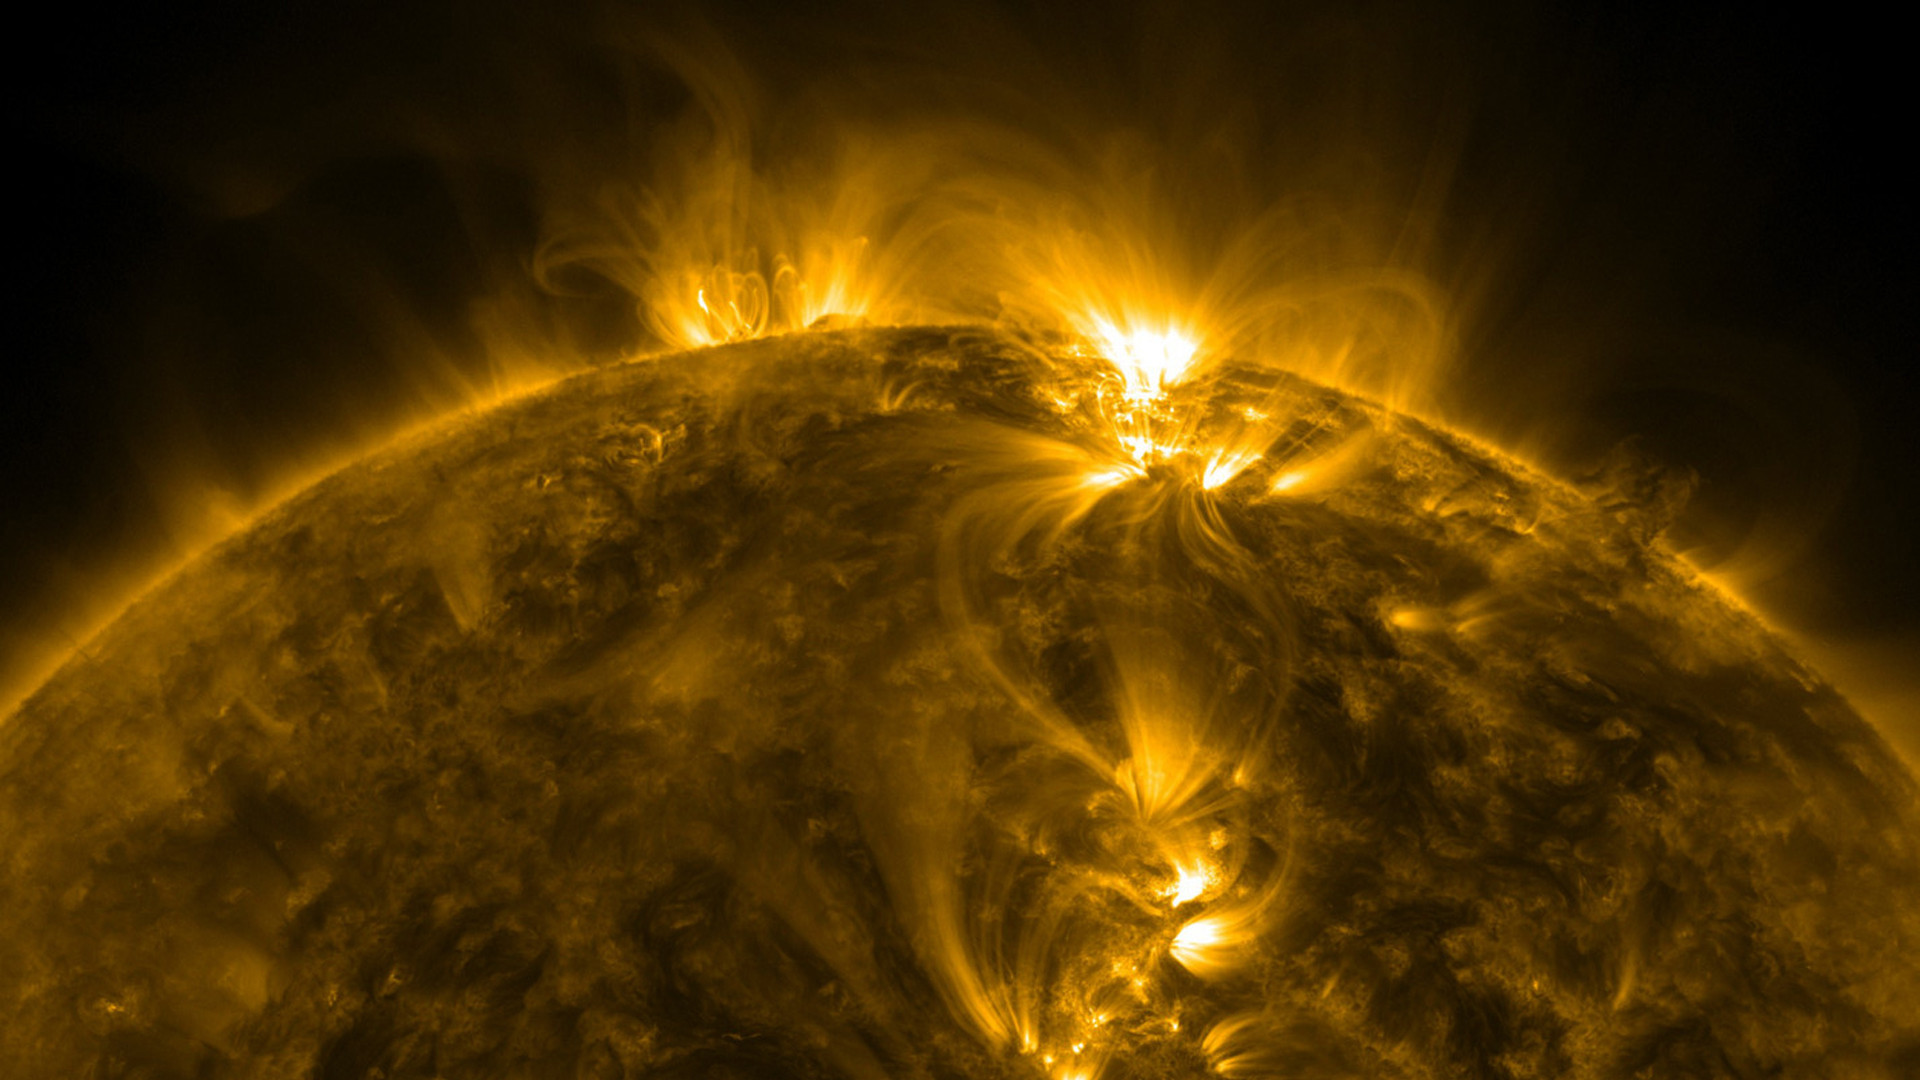
\includegraphics[scale=0.15]{media/main_sequence_stars.jpg}
\column{0.5\textwidth}
{\small
\textcolor{yellow}{\bf Velkommen til forelesning 2 av 2 for del 3D! I den første forelesningen så vi litt på stjernenes plasser i HR-diagrammet og hva det innenbærer at stjernene er på hovedserien. Nå skal vi se hva som skjer i alderdommen.{\large \textcolor{red}{Den første forelesningen i del 3D tar normalt ca. 1 time i den fysiske forelesningen, dvs. halvparten av en dobbelttime. Den andre delen av del 3D er lenger og tar normalt en hel dobbeltime.}}}\\
\textcolor{yellow}{(Illustrasjon: Solen observert med Solar Dynamics Observatory (Image: NASA/SDO))}}
\hyperlink{msx1}{\pagebutton{Neste side}}
\end{columns}
\end{frame}
}

\fullframe{msx1}{feil_intro}{riktig_ms1}{0}{
\huge
{\bf HUSK:} som vi sa i slutten av forrige forelesning, så trenger denne forelesningen {\bf forberedelse}: Du må lese og lære så godt du kan underavsnitt 3 om ``From the main sequence to the giant stage'' i \href{https://www.uio.no/studier/emner/matnat/astro/AST2000/h20/undervisningsmateriell/lecture_notes/part3d.pdf}{del 3D}.\\
\vspace*{1cm}
\textcolor{red}{Hvor var vi igjen i siste forelesning? La oss begynne med siste side av forrige forelesning...}
}{SIDE 1/6/57}

\colfullframe{riktig_ms1}{msx1}{ms2}{0}{yellow}{
Det er {\bf helt riktig!}.
\[
P=\frac{\rho kT}{\mu m_H}
\]
Her {\bf øker} jo $\mu$ ettersom vi få mer og mer helium. Husk at $\mu$ er et mål på midlere masse til atomkjernene, hvis vi får mer helium som er tyngre og mindre hydrogen etter kjernereaksjoner så må $\mu$ øke! Fra tilstandslikningen ser vi at {\bf hvis $\mu$ øker, så må trykket minke.} Og hvis trykke blir mindre, {\bf så vinner gravitasjon litt!} Og hvis gravitasjons da klarer å presse stjernen litt mer sammen så vil {\bf radien med tiden bli litt mindre.}. Stjernen krymper litt på hovedserien, men på meget sakte tidsskala. \textcolor{red}{Men hvor lenge holder den på med dette da? Hvor lenge lever stjernen på hovedserien? Det må vel være til den har brukt opp alt hydrogenet i de sentrale delene av stjernen der fusjonsreaksjonene foregår, men {\bf hvor lang tid} tar dette?}
}{SIDE 2/6/57}


\fullframenotxt{ms2}{riktig_ms1}{ms3}{0}{
  Vi skal på de neste sidene gjøre {\bf overslagsregning} for å finne ut hvor lenge en stjerne lever på hovedserien. Vi skal mikse samen masse forskjellige uttrykk og bruke de {\bf villeste antakelser} for å gjøre det lett å regne og {\bf kommer frem til sammenhenger som stemmer ganske godt med det man finner i avanserte datasimuleringer} av stjerner og med det man observerer! \textcolor{red}{Hvis du ikke har planer om å gjøre karriere som forsker i astrofysikk, så tenker du kanskje at dette er helt irrelevant for deg?} {\bf Da tar du grundig feil. For mange av dere som skal ut i ``vanlige'' jobber, så er det som vi gjør på de neste sidene sannsynligvis noe av det mest arbeidslivsrelevante dere gjør i bacheloren.} \hyperlink{ms2_b}{\pagebutton{\small Den må du lenger ut på landet med!}}
  \textcolor{white}{
Vel, mange av dere kommer til å jobbe med {\bf modellering} av komplekse systemer, det kan være veldig forskjellige systemer fra modellering av trafikken på veiene eller modellering av fisk og småkryp i en elv (eksempler på jobber som tidligere masterstudenter i astronomi faktisk gjør). Modellering av komplekse systemer kan være svært vanskelig hvis du ikke først finner noen virkelig kraftige men likevel ikke helt gale antakelser...}
}{SIDE 3/6/57}

\fullframe{ms2_b}{riktig_ms1}{ms3}{0}{
Vi skal på de neste sidene gjøre {\bf overslagsregning} for å finne ut hvor lenge en stjerne lever på hovedserien. Vi skal mikse samen masse forskjellige uttrykk og bruke de {\bf villeste antakelser} for å gjøre det lett å regne og {\bf kommer frem til sammenhenger som stemmer ganske godt med det man finner i avanserte datasimuleringer} av stjerner og med det man observerer! \textcolor{red}{Hvis du ikke har planer om å gjøre karriere som forsker i astrofysikk, så tenker du kanskje at dette er helt irrelevant for deg?} {\bf Da tar du grundig feil. For mange av dere som skal ut i ``vanlige'' jobber, så er det som vi gjør på de neste sidene sannsynligvis noe av det mest arbeidslivsrelevante dere gjør i bacheloren.} {\pagebutton{\small Den må du lenger ut på landet med!}}
Vel, mange av dere kommer til å jobbe med {\bf modellering} av komplekse systemer, det kan være veldig forskjellige systemer fra modellering av trafikken på veiene eller modellering av fisk og småkryp i en elv (eksempler på jobber som tidligere masterstudenter i astronomi faktisk gjør). Modellering av komplekse systemer kan være svært vanskelig hvis du ikke først finner noen virkelig kraftige men likevel ikke helt gale antakelser...
}{SIDE 3/6/57}






\fullframenotxt{ms3}{ms2}{ms4}{1}{
...og du må ofte kombinere forskjellige grener av fysikken eller også helt andre fagfelt for dermed å komme frem til en sterkt forenkelt modell. {\bf Dette er snakk om teft, det å ha gjort det mange ganger på mange forskjellige systemer!} \hyperlink{ms3_b}{\pagebutton{Ok, men hva skal man med en slik forenklet modell da?}} \textcolor{white}{Når du har funnet en slik sterkt forenklet modell, kan du\\
begynne å finne enkle sammenhenger som gjør at du får litt fysisk intuisjon for systemet ditt\\
bruke denne som grunnlag for en langt mer kompleks og realistisk modell/simulering\\
bruke denne til å teste den mer kompliserte modellen i enkle tilfeller\\
}
}{SIDE 4/6/57}

\fullframe{ms3_b}{ms2}{ms4}{1}{
...og du må ofte kombinere forskjellige grener av fysikken eller også helt andre fagfelt for dermed å komme frem til en sterkt forenkelt modell. {\bf Dette er snakk om teft, det å ha gjort det mange ganger på mange forskjellige systemer!} {\pagebutton{Ok, men hva skal man med en slik forenklet modell da?}} Når du har funnet en slik sterkt forenklet modell, kan du
\begin{itemize}
\item begynne å finne enkle sammenhenger som gjør at du får litt fysisk intuisjon for systemet ditt
\item bruke denne som grunnlag for en langt mer kompleks og realistisk modell/simulering
\item bruke denne til å teste den mer kompliserte modellen i enkle tilfeller
\end{itemize}
}{SIDE 4/6/57}




\fullframe{ms4}{ms3}{ms4b}{2}{
Med master i fysikk/astrofysikk blir du ofte ansatt nettopp for at du har erfaring med en slik prosess, ikke bare fordi du kan programmere for å løse problemer med datamaskin. Til det siste ansetter de like gjerne en informatiker. {\bf Det en fysiker har å tilby i tillegg er nettopp denne forståelsen av store og komplekse systemer, det å kunne bruke fysisk forståelse til å finne gode forenklinger, antakelser og sammenhenger som gjør at du kan forstå og beskrive systemet på en enkel måte.} \textcolor{red}{{\bf Det er akkurat det vi skal gjøre nå på de neste sidene...}}
}{SIDE 5/6/57}

\fullframe{ms4b}{ms4}{blue_nytema1}{0}{
\textcolor{red}{... så følg godt med og prøv å tenke deg at du har blitt ansatt av et firma som har en utmerket ide: å lage en kjempestor gasskule der hydrogenfusjon brukes til å lage energi. Før milliarder av kroner brukes på å konstruere denne gasskula, skal du bruke det du kan om fysikk til å gjøre overslag for å finne ut f.eks. hvor mye energi vi kan få og hvor lang levetid en slik fusjonsreaktor vil kunne ha. Og spesielt hvor stor masse bør en slik kule ha for å optimalisere energien vi utvinner? Hva er sammenhengen mellom massen og energien vi får?}
}{SIDE 6/6/57}

\renewcommand{\headline}{Levetid på hovedserien}
{
\setbeamercolor{background canvas}{bg=blue}
\begin{frame}
\label{blue_nytema1}
\hyperlink{ms4b}{\pagebutton{\small Forrige side}}
\nytemaside{farvel}
\textcolor{yellow}{Du får nå en laaaaaaaang utledning. Har du en kaffemaskin i nærheten? Har du sovet godt? Er hjernen klar? {\bf Hvis svaret er nei på noen av disse spørsmålene, bør du vente med dette til du er klar!} Men frykt ikke, vi skal ta en pause omtrent midtveis, men ta gjerne flere på eget initiativ.}
\hyperlink{ms5}{\pagebutton{OK, jeg trekker pusten godt nå og er klar...}}
\end{frame}
}


\fullframenotxt{ms5}{ms4b}{red_ms6}{0}{
La oss begynne med et enkelt spørsmål først. Anta at du kjenner massem $M$ til gasskula (aka stjerna), at fusjonsreaksjoner kun foregår i kjernen som utgjør en andel $p$ av massen til kula. Anta videre at vi kjenner luminositeten $L$. Kan du finne et uttrykk for hvor lenge denne stjerna kommer til å produsere energi ved at hydrogen fusjonener til helium?\hyperlink{ms5_b}{\pagebutton{Jeg har skrevet ned et forslag}}
\textcolor{white}{
Så total masse som blir fusjonert er $pM$. Masse går over til energi via uttrykket $E=mc^2$ der $c$ er lysfarten, så total energi som blir produsert i løpet av hele stjerna (unnskyld, gasskula) sin levetid må være $E=pMc^2$. Og energien som produseres per tid er $L$. Da må vel levetiden bli
\[
t_\mathrm{life}=\frac{pMc^2}{L}
\]
Ok, da mangler vi ``bare'' luminositeten $L$ for å finne levetida. Men det er ikke bare-bare...}
}{SIDE 7/45/57}

\fullframe{ms5_b}{ms4b}{red_ms6}{0}{
La oss begynne med et enkelt spørsmål først. Anta at du kjenner massem $M$ til gasskula (aka stjerna), at fusjonsreaksjoner kun foregår i kjernen som utgjør en andel $p$ av massen til kula. Anta videre at vi kjenner luminositeten $L$. Kan du finne et uttrykk for hvor lenge denne stjerna kommer til å produsere energi ved at hydrogen fusjonener til helium?{\pagebutton{Jeg har skrevet ned et forslag}}
Så total masse som blir fusjonert er $pM$. Masse går over til energi via uttrykket $E=mc^2$ der $c$ er lysfarten, så total energi som blir produsert i løpet av hele stjerna (unnskyld, gasskula) sin levetid må være $E=pMc^2$. Og energien som produseres per tid er $L$. Da må vel levetiden bli
\[
t_\mathrm{life}=\frac{pMc^2}{L}
\]
Ok, da mangler vi ``bare'' luminositeten $L$ for å finne levetida. Men det er ikke bare-bare...
}{SIDE 7/45/57}







\colfullframe{red_ms6}{ms5}{red_ms7}{1}{red}{
\textcolor{yellow}{\Huge
For hvordan kan du lage et overslag for luminositeten til en fusjonerende gasskule? Du kan anta at du kjenner massen og radien. Du kjenner ikke levetida. Hvor begynner du? Si at du kan anta de aller villeste forenklinger, kan du da komme på noen forslag?
}
}{SIDE 8/45/57}

\colfullframe{red_ms7}{red_ms6}{red_ms7b}{0}{red}{
\textcolor{yellow}{\Huge
Har du fått ned noen ideer på papiret? Du kan jo ikke få sparken allerede før du har begynt! {\bf Noe, må du kunne vise frem for at firmaet enda skal ha tiltro til deg.}
}
}{SIDE 9/45/57}


\colfullframe{red_ms7b}{red_ms7}{ms8}{0}{red}{
\textcolor{yellow}{\Huge
Ta ihvertall 5-10 minutter, diskuter med medstudenter og skriv ned i det minste noen konsepter eller bruddstykker av ideer og ting som du kanskje kunne bruke på en eller annen måte. {\bf NOE må du få ned på papiret}. Det står om karrieren din!
}
}{SIDE 10/45/57}


\fullframe{ms8}{red_ms7b}{ms9}{0}{
Allright, la oss prøve å dele opp problemet litt, det pleier å være et godt startpunkt. Vi vet at luminositet er definert som
\[
L=\frac{\Delta E}{\Delta t}
\]
La oss tenke oss at vi kan slå av og på kjernereaksjonene i sola, ok? Vi slår de på et kort lite øyeblikk og får produsert en energi $\Delta E$ i løpet av dette øyeblikket. Og så {\bf venter vi!}. Vi venter til all denne energien har kommet frem til overflaten av sola og blitt strålt ut. Det tar langt tid, husk at radien til sola er 800.000 km!. Anta at vi finner tiden $\Delta t$. Da kan vi putte inn i formelen over her for å finne luminositeten. En energi $\Delta E$ som ble {\bf strålt ut} i løpet tiden $\Delta t$. Og slik holder vel sola egentlig på hele tida? I hvert lite øyeblikk lager den energi $\Delta E$ som trenger tiden $\Delta t$ på å komme ut. Hvis vi finner $\Delta E$ og $\Delta t$, så har vi luminositeten!
}{SIDE 11/45/57}


\fullframe{ms9}{ms8}{ms10}{0}{\small
Før vi kan se noe nærmere på det, må vi nesten se hvordan energien transporteres fra sentrum av en stjerne og opp til overflaten. Det finnes 3 hovedprosesser for energitransport gjennom et medium:
\begin{itemize}
\item {\bf Energitransport ved stråling:} Her er det rett og slett fotoner som beveger seg utover og tar med seg energien. Tenk deg en glødende varmeovn, varmestrålingen treffer deg og avgir energien. Energien transporteres gjennom lufta til deg.
\item {\bf Energitransport ved konveksjon:} Konveksjon er når varm gass/væske beveger seg opp til områder der gassen/væsken er kaldere og avgir energi. Tenk deg en kokeplate: vannet i bunnen av kjelen varmes opp, den flyter opp (kokebobler!) til de kaldere områdene og avgir varme. Energien transporteres oppover i kjelen
\item {\bf Energitransport ved konduksjon:} Tilbake til kjelen over: anta at du setter den på kokeplata uten vann i. Da transporteres varmen gjennom metallet, gjennom en kjedereaksjon av kollisjoner mellom atomer i metallet. Dermed blir også de øvre delene av kjelen som ikke er i kontakt med plata varm. Energien transporteres gjennom metallet i kjelen.
\end{itemize}
}{SIDE 12/45/57}

\fullframe{ms10}{ms9}{red_ms11}{0}{\small
I {\bf stjerner} er det hovedsaklig energitransport ved {\bf stråling og/eller ved konveksjon}. Energien kan transporteres fra kjernen via fotoner eller via gassmasser som beveger seg oppover i stjerna akkurat som kokeboblene. I sola så foregår energitransport ved stråling opp til ca. $0.7R_\odot$ og deretter ved konveksjon opp til overflaten. Her ser du bilde av konveksjonscellene (kokeboblene) på solas overflate:\\
\centerline{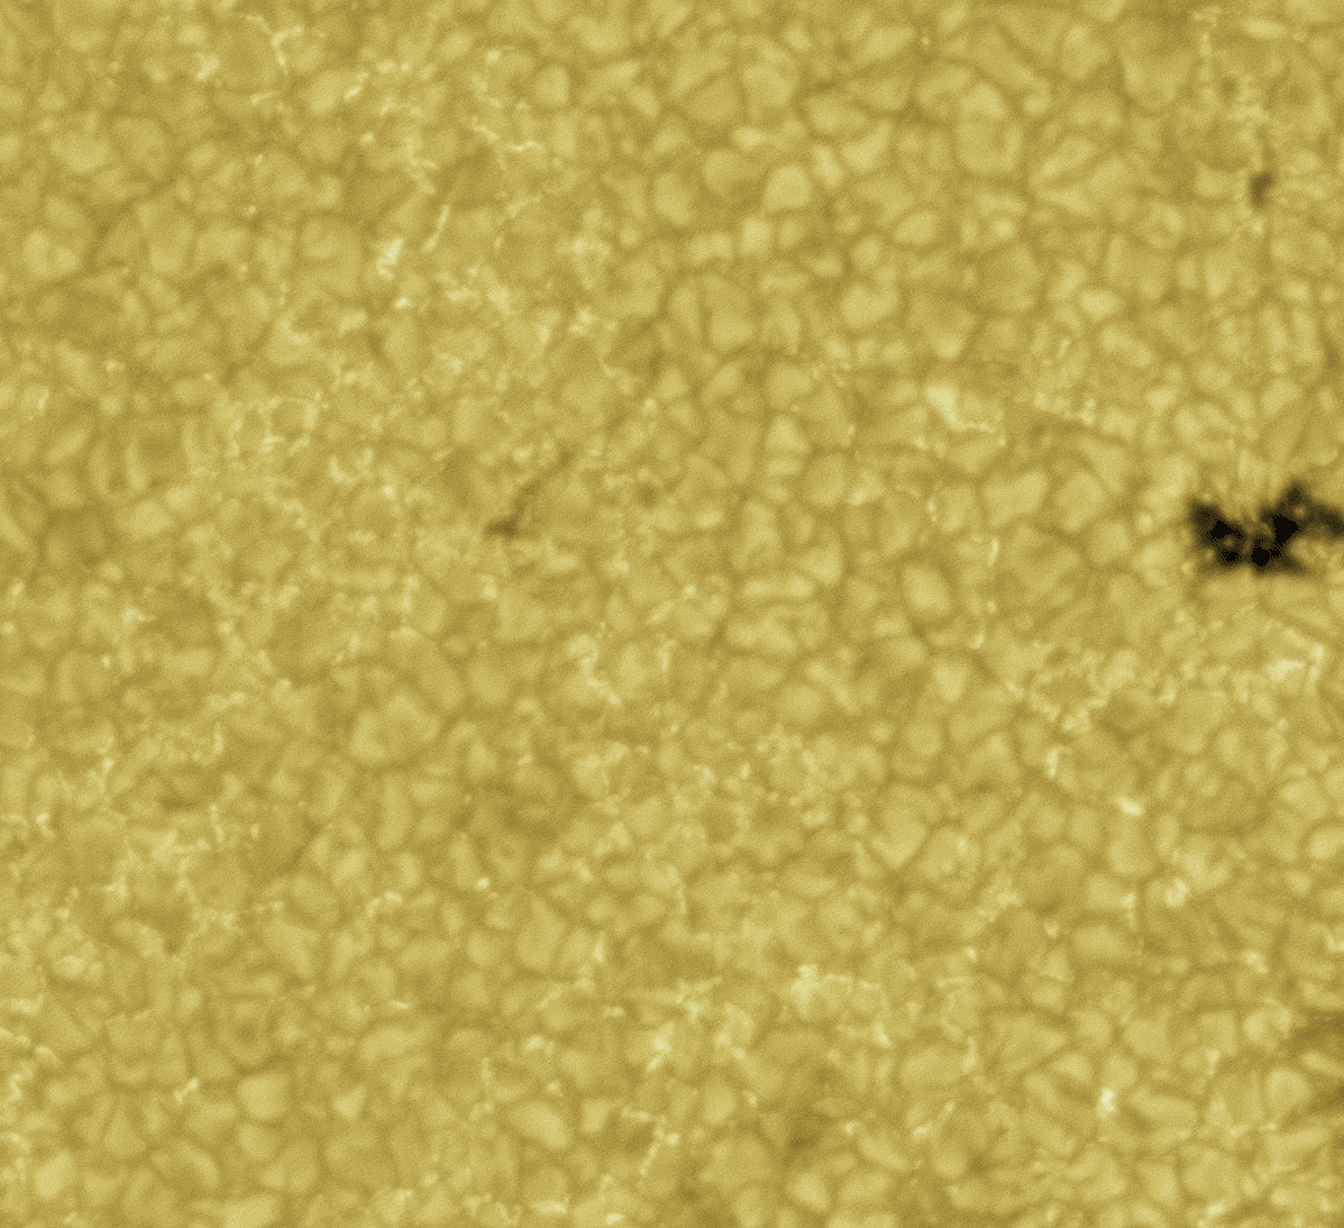
\includegraphics[scale=0.22]{media/convection.png}}
Du kan se tilsvarende \href{https://www.nasa.gov/sites/default/files/thumbnails/image/convectivecells.gif}{video} her. (Credits: NASA/JAXA/Hinode)
}{SIDE 13/45/57}

\colfullframe{red_ms11}{ms10}{ms12}{0}{red}{
\textcolor{yellow}{\Huge
En av antakelsene våre skal være at all transport skjer med stråling. Det er lettere å ha kontroll på fotoner som beveger seg utover enn store gassmasser. Da er vi klare her til å prøve å finne hvor stor energi $\Delta E$ som trenger tid $\Delta t$ på å komme seg ut av sola. Og derav finne Luminositeten...}
}{SIDE 14/45/57}





\fullframe{ms12}{red_ms11}{ms12b}{0}{
La oss begynne med energien $\Delta E$ som forlater stjerna. Den energien som frigjøres i fusjonsreaksjonene omgjøres til kinetisk energi for partiklene i kjernen av stjerna samt stråling. Det blir til slutt en likevekt mellom fotonene (strålingen) og gasspartiklene. Fusjonsreaksjonene varmer på den måten opp kjernen til en kjernetemperatur $T_c$ (``C'' for Core, kjernen er hele det sentrale området av stjerna der fusjon foregår). {\bf Vi ser på kjernen som et sort legeme som sender ut termisk stråling på temperatur $T_c$,  Planck-stråling!}. Ved så høy temperatur som vi har i kjernen av en stjerne så blir {\bf denne sorte strålingen intens} Bare prøv å tegne Plancks strålingskurve for en temperatur på flere milllioner grader, eller se på fluksen fra Stefan Boltzmann, eller Wiens forskyvningslov, hvilke bølgelenger får vi fra et sort legeme med så høy temperatur?
}{SIDE 15/45/57}

\fullframe{ms12b}{ms12}{red_ms13}{0}{
Ved så høy temperatur blir det så mange fotoner i de sentrale delene av en stjerne at vi snakker om en {\bf fotongass}. Rett og slett massevis av fotoner som svirrer rundt og kolliderer med gasspartikler. Fotonene oppfører seg dermed selv som gasspartikler og vi kan med rette bruke begrepet fotongass. En {\bf stjernes kjerne består dermed av varm hydrogen(++)gass blandet med denne fotongassen.} \textcolor{red}{Vi har altså hele tiden et energireservoar i stjernens kjerne i form av fotoner.} {\bf I termodynamikken kommer du til å lære at energitettheten $\rho_E$ (energi per $\mathrm{m}^3$) i en fotongass er gitt ved $\rho_E=aT^4$} der $a$ er strålingskonstanten (husker du fra \href{https://www.uio.no/studier/emner/matnat/astro/AST2000/h20/undervisningsmateriell/lecture_notes/part3d.pdf}{del 1E} at trykket i en fotongass er $P=\frac{1}{3}aT^4$?). (Og $T^4$ for et sort legeme kan du kanskje tippe hvor kommer fra?)
}{SIDE 16/45/57}


\colfullframe{red_ms13}{ms12b}{red_ms14}{0}{red}{
\textcolor{yellow}{\Huge
Hvis vi antar at kjernen til stjerna har en radius $R_c$, har du nå kommet noe nærmere hvordan du kan gå frem for å finne luminositeten?? Hva kan vi bruke som denne energi $\Delta E$ som skal slippe ut i løpet av tiden $\Delta t$?
}
}{SIDE 17/45/57}

\colfullframe{red_ms14}{red_ms13}{ms15}{0}{red}{
\textcolor{yellow}{\Huge
Hvis du ikke nå har kommet {\bf noe} nærmere løsningen. Anta at vi nå skrur av alle kjernereaksjoner i sola. Hvor mye energi $\Delta E$ kommer den til å stråle ut før den slukner?
}
}{SIDE 18/45/57}

\fullframenotxt{ms15}{red_ms14}{ms16}{0}{
Med energitetther $\rho_E=aT_c^4$ og kjerneradius $R_c$ så får vi vel at den totale energien i en stjernes kjerne i fotoner til enhver tid er gitt ved
\[
E=\frac{4}{3}\pi R_c^3aT_c^4
\]
{\bf Her har vi allerede gjort en stor antakelse, kan du se hvilken?}\hyperlink{ms15_b}{\pagebutton{Tjaaaaa....}} \textcolor{white}{Tror du virkelig temperaturen og dermed energitettheten er den samme gjennom hele kjernen? Det er vel en ganske grov antakelse?\\
{\bf OK, her er planen:} Slår vi av kjernereaksjoner, så er det energien $\Delta E$ i alle disse fotonene som er igjen å stråle ut av sola. Det store spørsmålet hvor lang tid $\Delta t$ denne energien, altså alle disse fotonene trenger for å komme frem til solas overflate? Har vi det, har vi luminositeten $L=\Delta E/\Delta t$. {\Large\bf Noen forslag til hvor vi kan starte for å finne ut hvor lang tid fotonene trenger for å komme seg ut?}}
}{SIDE 19/45/57}

\fullframe{ms15_b}{red_ms14}{ms16}{0}{
Med energitetther $\rho_E=aT_c^4$ og kjerneradius $R_c$ så får vi vel at den totale energien i en stjernes kjerne i fotoner til enhver tid er gitt ved
\[
E=\frac{4}{3}\pi R_c^3aT_c^4
\]
{\bf Her har vi allerede gjort en stor antakelse, kan du se hvilken?}{\pagebutton{Tjaaaaa....}} \textcolor{red}{Tror du virkelig temperaturen og dermed energitettheten er den samme gjennom hele kjernen? Det er vel en ganske grov antakelse?}\\
{\bf OK, her er planen:} Slår vi av kjernereaksjoner, så er det energien $\Delta E$ i alle disse fotonene som er igjen å stråle ut av sola. Det store spørsmålet hvor lang tid $\Delta t$ denne energien, altså alle disse fotonene trenger for å komme frem til solas overflate? Har vi det, har vi luminositeten $L=\Delta E/\Delta t$. {\Large\bf Noen forslag til hvor vi kan starte for å finne ut hvor lang tid fotonene trenger for å komme seg ut?}
}{SIDE 19/45/57}





\fullframe{ms16}{ms15}{red_ms16b}{1}{
{\bf Ikke det??} La oss ta det litt rolig her: Anta at et foton hele tiden kolliderer med gasspartikler og skifter retning. Den midlere veilengden som et foton går mellom hver kollisjon kaller vi $\ell$. Hvor mange kollisjoner $N$ får et foton før det når overflaten av stjerna? Klarer du å vise at det er
\[
N=\frac{R^2}{\ell^2}
\]
??? Og gitt dette, klarer du å vise at fotonet i gjennomsnitt trenger en tid
\[
\Delta t=\frac{R^2}{\ell c}
\]
der $c$ er lyshastigheten til å komme seg opp til overflaten?
{\bf Her bør du sette av 5-10 minutter til å se om du klarer å komme i mål selv. Spesielt det siste uttrykket bør du får til, gitt at du kjenner det første. Det første uttrykket er noe mer tricky, men ikke mer enn at du ihvertfall bør kunne sette opp starten av utregningen (og en tegning av fotonets vei fra stjernas sentrum og ut vil hjelpe mye!}.
}{SIDE 20/45/57}


\colfullframe{red_ms16b}{ms16}{red_ms16b2}{0}{red}{
\textcolor{yellow}{\Huge
Har du gjort et skikkelig forsøk og kommet et stykke på vei? Hvis ikke, gå tilbake og prøv igjen, {\bf noe må du få til} for a betrygge arbeidsgiveren din her om at du jobber med saken!}
}{SIDE 21/45/57}

\fullframe{red_ms16b2}{red_ms16b}{ms16c}{0}{{\Huge
Hjelper denne figuren deg???
\centerline{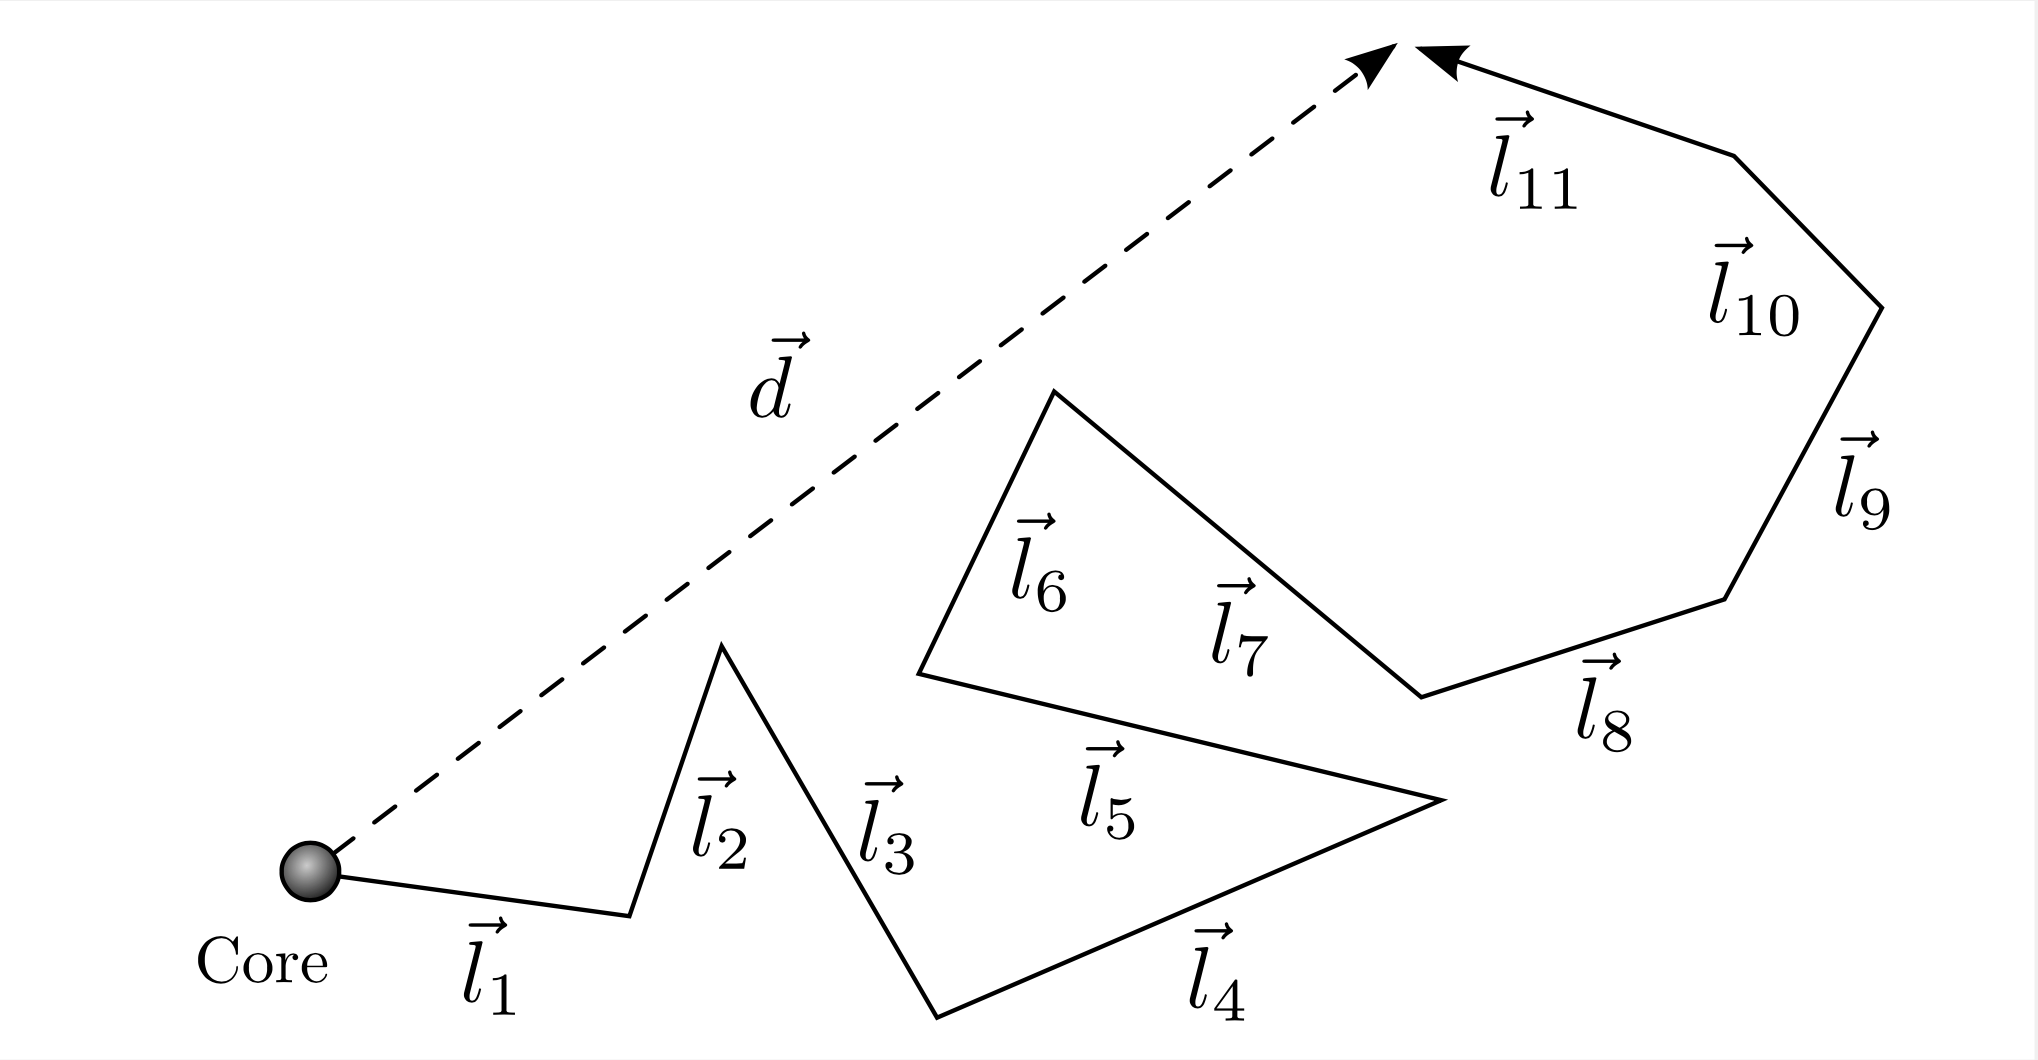
\includegraphics[scale=0.7]{media/fig_20-2.png}}}
}{SIDE 22/45/57}


\fullframe{ms16c}{red_ms16b2}{red_ms17}{0}{
Se \href{https://www.uio.no/studier/emner/matnat/astro/AST2000/h20/undervisningsmateriell/interaktive-forelesningsnotater/3d/videoer/video3d_1.mp4}{denne videoen} her for å sette sammen bitene og finne ut hvorfor
\[
N=\frac{R^2}{\ell^2}
\]
og
\[
\Delta t=\frac{R^2}{\ell c}
\]
Henger du med? Kan du nå skrive ut uttrykk for luminositeten $L$ ved hjelp av de størrelsene du har nå?
}{SIDE 23/45/57}


\colfullframe{red_ms17}{ms16c}{ms18}{0}{red}{
\Large
\textcolor{yellow}{Nå begynner moroa her! Nå skal du gjøre noe som man alltid må gjøre når man prøver å forstå et komplekst system.} {\bf Med alle tilnærmingene vi gjør og med den fulle kompleksiteten til systemet så har vi ingen sjans til å finne uttrykk med presise tallstørrelser.} \textcolor{yellow}{Det vi kan finne, og som kan være minst like interessant som tallstørrelser er {\bf proporsjonaliteter}.} {\bf Dvs. f.eks. hvordan endrer luminositeten eller stjernas levetid seg som funksjon av totalmassen? Altså hvis vi dobbler massen, hva skjer med luminositeten?} \textcolor{yellow}{Dette vil si oss veldig mye om effektiviteten til gasskula vår selv om vi ikke nødvendigvis får ut eksakte tall for luminositeten!}
}{SIDE 24/45/57}


\fullframe{ms18}{red_ms17}{ms19}{0}{
\Large
Denne typen fysikk-overslagsregning er ikke bare noe man driver med i arbeidslivet, det er også noe en forsker i fysikk driver med hele tiden, og du kommer til å bruke det i masteroppgaven. Dette er kanskje litt uvant da de første semesterne i fysikkstudiet ofte blir brukt til mye eksakt (men urealistisk) regning. {\bf Da var det jaggu på tide at du får prøve deg her!} Fra det vi har gjort så langt, vis at luminositeten til stjerna kan skrives med følgende proporsjonalitet (legg merke til $\propto$ tegnet for proporsjonalitet)
\[
L\propto RT_c^4\ell
\]
Hvis du tviler, ta en titt på \href{https://www.uio.no/studier/emner/matnat/astro/AST2000/h20/undervisningsmateriell/interaktive-forelesningsnotater/3d/videoer/video3d_2.mp4}{denne videoen}
}{SIDE 25/45/57}


\fullframe{ms19}{ms18}{ms20}{0}{
Hva med den midlere veilengden $\ell$ for fotonet? Den avhenger at {\bf en} enkelt egenskap ved gassen. {\bf\Large Hvilken? Og hva er proporsjonaliteten??}. Prøv å tegne en boks med gasspartikler, fordel partiklene så jevnt utover i boksen som mulig. Tegn inn et foton et sted i midten. Hvilken egenskap ved gassen avgjør hvor langt fotonet i gjennomsnitt kan bevege seg før det kolliderer? Og hvordan kan du nå skrive proporsjonaliteten med denne egenskapen, altså
\[
\ell\propto??
\]
Ikke bla om før du har gjort et skikkelig forsøk.
}{SIDE 26/45/57}


\choiceframe{ms20}{ms19}{0}{
Blir det
\hyperlink{feil_ms20b}{\choicebutton{$\ell\propto T^2$}}
\hyperlink{feil_ms20b}{\choicebutton{$\ell\propto P$}}
\hyperlink{feil_ms20b}{\choicebutton{$\ell\propto \rho^2$}}
\hyperlink{feil_ms20b}{\choicebutton{$\ell\propto \frac{1}{T}$}}
\hyperlink{feil_ms20b}{\choicebutton{$\ell\propto \frac{1}{P^2}$}}
\hyperlink{riktig_ms20c}{\choicebutton{$\ell\propto \frac{1}{\rho}$}}
\hyperlink{feil_ms20b}{\choicebutton{$\ell\propto \frac{1}{\rho^3}$}}
\hyperlink{feil_ms20b}{\choicebutton{$\ell\propto T^4$}}
der $P$, $T$ og $\rho$ er henholdsvis trykk, temperatur og massetetthet til gassen (ikke fotongassen men hydrogengassen)
}{SIDE 27/45/57}


\colchoiceframe{feil_ms20b}{ms20}{0}{black}{\Large
\textcolor{yellow}{
Det ble nok ikke rett! Har du tegnet opp partiklene? Har du prøvd med en ny tegning når du f.eks. har dobblet størrelsen på den egenskapen ved gassen som du tror er viktig her? Har du sett hvordan $\ell$ da bør endre seg? Hvis du har kommet hit for andre gang, se på \href{https://www.uio.no/studier/emner/matnat/astro/AST2000/h20/undervisningsmateriell/interaktive-forelesningsnotater/3d/videoer/video3d_3.mp4}{denne videoen}}
}{SIDE 28/45/57}


\colfullframe{riktig_ms20c}{ms20}{pause}{-1}{yellow}{\Huge
Det er helt riktig! Hvis du enda er usikker, ta en titt på  \href{https://www.uio.no/studier/emner/matnat/astro/AST2000/h20/undervisningsmateriell/interaktive-forelesningsnotater/3d/videoer/video3d_3.mp4}{denne videoen}. Kan du nå vise at
\[
L\propto\frac{R^4T_c^4}{M}
\]
??? Det bør du få til nå, hvis ikke, spør foreleser!
}{SIDE 29/45/57}

{
\setbeamercolor{background canvas}{bg=cyan}
\begin{frame}
\label{pause}
\hyperlink{riktig_ms20c}{\pagebutton{\small Forrige side}}
{\large
\centerline{{Eeeeeeendlig kaffe!}}
\centerline{
\includegraphics[scale=4]{media/drink-coffee.png}}\\
{med mye sukker! Og jammen bør du ta en tur bortom kantina eller kiosken og se om de har en sjokoladebit eller kakebit? Det har du fortjent nå. {\bf Ihvertfall bør du ta turen om du så ikke kjøper noe, en luftetur er påkrevet før du fortsetter!}
\vspace*{0.5cm}
Ikke lov å fortsette før du har tatt minst 15 min. pause!}
}\\
\vspace*{0.5cm}
\hyperlink{ms20d}{\pagebutton{Allright, alltright, jeg tror jeg er klar for resten...}}
\end{frame}
}

\fullframe{ms20d}{riktig_ms20c}{ms20e}{0}{
La du merke til hvilken vannvittig antakelse du brukte her?? Du antok at tettheten til stjerna er den samme gjennom hele stjerna, altså uniform tetthet! Det er ikke veldig realistisk, men tettheten vil jo være tettere enn dette i kjernen og tynnere enn dette mot overflaten, kanskje det blir ok i gjennomsnitt likevel?\\
Vi har nå altså en proporsjonalitet
\[
L\propto\frac{R^4T_c^4}{M}
\]
for luminositeten som funksjon av massen og radien til stjerna i tillegg til kjernetemperaturen $T_c$.
}{SIDE 30/45/57}

\fullframe{ms20e}{ms20d}{ms21}{0}{
\textcolor{red}{Men det er vital informasjon som vi ikke har brukt! \bf Og her kommer et annet viktig punkt når det kommer til fysikk-overslagsregning: du må få med all informasjonen du har om systemet!}\\
 {\Huge Kan du tenke deg noen sammenhenger som vi kjenner til men enda ikke har benyttet? Det er flere enn en!} Ikke gå videre før du har skrevet ned minst en ting til som du vet om dette systemet og som kan være bruklig for å komme frem til en enda enklere sammenheng for luminositeten!
}{SIDE 31/45/57}


\fullframe{ms21}{ms20e}{ms21b}{0}{
{\Large Hadde du hydrostatisk likevekt på lista di?}
Kan du vise at likningen for hydrostatisk likevekt kan gi deg en sammenheng alla
\[
P_c\propto\frac{M^2}{R^4}
\]
der $P_c$ er trykket i kjernen??? Du skal snart få tenke videre på denne, men la oss ta det litt videre først!
Husk at det vi ønsker nå er å få proporsjonaliteten
\[
L\propto\frac{R^4T_c^4}{M}
\]
så enkel som mulig!
}{SIDE 32/45/57}

\fullframe{ms21b}{ms21}{red_ms22}{0}{
Tenk deg altså at du har fått
\[
P_c\propto\frac{M^2}{R^4}
\]
fra hydrostatisk likevekt. Men hva hjelper det oss for å få proporsjonaliteten for $L$ enklere? \textcolor{red}{Nå har vi jo fått inn en ny variabel her, trykket $P$, og da blir det jo ikke enklere men vanskeligere!} MEN så finnes det en sammenheng til for gassen som du bør kunne tenke deg. En sammenheng mellom blant annet trykk og temperatur slik at vi blir kvitt trykket i uttrykket her, får inn $T_c$ isteden, og dermed kvitter oss med $T_c$ i uttrykket på forrige side. Da snakker vi om forenklinger da! {\bf Kan du vise, ved å sette inn denne sammenhengen for $P$ at vi da får en sammenheng som sier}
\[
T_c\propto\frac{M}{R}
\]
som altså er veldig fristende å bruke for å kvitte oss med $T_c$ i uttryket for $L$ på forrige side.
}{SIDE 33/45/57}





\colfullframetxt{red_ms22}{ms21b}{ms23}{0}{red}{Jeg har kommet et stykke på vei ihvertfall}{\textcolor{yellow}{\Large
Tilbake til proporsjonaliteten for $P$ som du skal finne fra hydrostatisk likevekt...
Fikk du det til? Det er ikke lov å gå videre uten å ha noe forslag, selv om du ikke kommer helt frem. Nå er vi nesten fremme ved det endelige uttrykket her. Firmaet vi jobber for begynner å blir riktig så fornøyd, dette ser lovende ut, vi har nesten gjort jobben vår som en god fysiker! Du kan ikke skuffe dem nå?}
}{SIDE 34/45/57}

\fullframe{ms23}{red_ms22}{ms24}{0}{\Large
I \href{https://www.uio.no/studier/emner/matnat/astro/AST2000/h20/undervisningsmateriell/interaktive-forelesningsnotater/3d/videoer/video3d_4.mp4}{denne videoen} ser du hvordan man kan gjøre forenklingen med hydrostatisk likevekt og hva den andre kjente sammenhengen var som gjør at vi kommer frem til at
\[
T_c\propto\frac{M}{R}
\]
som innsatt i
\[
L\propto\frac{R^4T_c^4}{M}
\]
gir oss...ja hva gir det...
}{SIDE 35/45/57}


\fullframe{ms24}{ms23}{ms25}{0}{\huge
Lo and behold, det gir oss
\[
L\propto M^3
\]
Så vanvittig enkelt? Et så komplekst system og en så enkel relasjon? Men hva sier de store avanserte datamodellene da? De som kjører på 1000-vis av prosessorer i flere måneder?
}{SIDE 36/45/57}


\fullframe{ms25}{ms24}{ms26}{0}{\Large
De sier
\[
L\propto M^\beta
\]
hvor $\beta$ avhenger litt av massen til stjerna. For stjerner med veldig stor masse, titalls solmasser, så passer $\beta=3$ slik vi fant ganske godt! Merk at slike stjerner har energitransport med stråling gjennom hele stjerna, akkurat slik som vi antok. \textcolor{red}{For stjerner med mindre masse slik som sola så er $\beta=4$ en bedre tilnærmelse. Den gjelder for flere stjerner, så vi skal bruke den i dette kurset.} {\Large\bf Men er det ikke helt utrolig at vi kom frem til nesten det samme med en utrolig enkel utledning med store og grove antakelser?}
}{SIDE 37/45/57}

\fullframe{ms26}{ms25}{ms26b}{0}{\Large
Hvilke antakelser var det vi gjorde igjen?
\begin{itemize}
\item energitransport med stråling gjennom hele stjerna (er sant for veldig massive stjerner)
\item uniform temperatur i hele stjernens kjerne (der det foregår kjernereaksjoner)
\item uniform tetthet gjennom hele stjerna
\item at trykket går som $P(r)\propto r^n$ gjennom hele stjerna
\item ideel gass
\end{itemize}
Pluss en del mer subtile antakelser som vi ikke nevner. Flere av disse antakelsene er ikke spesielt gode, men det at vi ser på et stort system, midler over størrelser som f.eks. både høyere og lavere tetthet enn den uniforme tettheten som vi antar, så kommer vi likevel frem til noe som stemmer godt med virkeligeheten.
}{SIDE 38/45/57}

\fullframenotxt{ms26b}{ms26}{ms27}{0}{
Så hva sier denne sammenhengen oss:
\[
L\propto M^4
\]
(som er den varianten som vi skal bruke siden den passer på langt flere stjerner enn $L\propto M^3$ som vi kom frem til med alle forenklingene våre)\\
En stjerne som er dobbelt så massiv som sola, hvor stor luminositet har den?\hyperlink{ms26b_b}{\pagebutton{Jeg har det, jeg har det!}}
\textcolor{white}{
Nettopp, ja 16 ganger mer energi per sekund enn sola. Og bare dobbel masse! {\bf Dette er jo vital informasjon} for arbeidsgiveren vår som skal bygge en fusjonsreaktor som er en stor gasskule! Jobben fullført! Ihvertfall den innledende fasen. Hvis behovet for energi er stort, så ha stor masse. {\bf Men det var en problemstilling til som vi begynte med, var det ikke? Hvor lenge lever en slik stjerne?}}
}{SIDE 39/45/57}

\fullframe{ms26b_b}{ms26}{ms27}{0}{
Så hva sier denne sammenhengen oss:
\[
L\propto M^4
\]
(som er den varianten som vi skal bruke siden den passer på langt flere stjerner enn $L\propto M^3$ som vi kom frem til med alle forenklingene våre)\\
En stjerne som er dobbelt så massiv som sola, hvor stor luminositet har den?{\pagebutton{Jeg har det, jeg har det!}}
Nettopp, ja 16 ganger mer energi per sekund enn sola. Og bare dobbel masse! {\bf Dette er jo vital informasjon} for arbeidsgiveren vår som skal bygge en fusjonsreaktor som er en stor gasskule! Jobben fullført! Ihvertfall den innledende fasen. Hvis behovet for energi er stort, så ha stor masse. {\bf Men det var en problemstilling til som vi begynte med, var det ikke? Hvor lenge lever en slik stjerne?}
}{SIDE 39/45/57}





\choiceframe{ms27}{ms26b}{1}{
Vi fant for en god del sider siden at
\[
t_\mathrm{life}=\frac{pMc^2}{L}
\]
Hvis vi igjen bare er interessert i proporsjonalitet, så tar vi denne videre:
\[
t_\mathrm{life}\propto???
\]
Ja, hvordan blir det?
\hyperlink{feil_ms27b}{\choicebutton{$t_\mathrm{life}\propto M$}}
\hyperlink{feil_ms27b}{\choicebutton{$t_\mathrm{life}\propto M^2$}}
\hyperlink{feil_ms27b}{\choicebutton{$t_\mathrm{life}\propto M^3$}}
\hyperlink{feil_ms27b}{\choicebutton{$t_\mathrm{life}\propto M^4$}}
\hyperlink{feil_ms27b}{\choicebutton{$t_\mathrm{life}\propto 1/M$}}
\hyperlink{feil_ms27b}{\choicebutton{$t_\mathrm{life}\propto 1/M^2$}}
\hyperlink{riktig_ms27c}{\choicebutton{$t_\mathrm{life}\propto 1/M^3$}}
\hyperlink{feil_ms27b}{\choicebutton{$t_\mathrm{life}\propto 1/M^4$}}
}{SIDE 40/45/57}


\colchoiceframe{feil_ms27b}{ms27}{0}{black}{\Large
\textcolor{yellow}{
Nei, det ble ikke rett! Er du enig i at
\[
t_\mathrm{life}=\frac{pMc^2}{L}\propto\frac{M}{L}
\]
Og hvis $L\propto M^4$, ja da bør du komme frem til ... gå tilbake og prøv igjen.
}
}{SIDE 41/45/57}


\colfullframenotxt{riktig_ms27c}{ms27}{ms28}{-1}{yellow}{\Large
Det er helt riktig! Kan du nå vise at
\[
t_\mathrm{life}\propto\frac{1}{M^3}
\]
Altså en stjerne som er dobbelt så massiv som solen vil leve i ...\hyperlink{riktig_ms27c_b}{\pagebutton{Shit! Strek i regningen!}}
\textcolor{yellow}{
Bare 1/8 av solas levetid? Tuller du? Da faller jo ideen i grus her, med stor masse får vi masse energi ut, men så blir fusjonsreaktoren ``brukt opp'' i løpet av en mye kortere tid!}
}{SIDE 42/45/57}

\colfullframe{riktig_ms27c_b}{ms27}{ms28}{-1}{yellow}{\Large
Det er helt riktig! Kan du nå vise at
\[
t_\mathrm{life}\propto\frac{1}{M^3}
\]
Altså en stjerne som er dobbelt så massiv som solen vil leve i ...\pagebutton{Shit! Strek i regningen!}
Bare 1/8 av solas levetid? Tuller du? Da faller jo ideen i grus her, med stor masse får vi masse energi ut, men så blir fusjonsreaktoren ``brukt opp'' i løpet av en mye kortere tid!
}{SIDE 42/45/57}





\fullframe{ms28}{riktig_ms27c}{ms29_0}{0}{\large
Når vi først er igang, så la oss gjøre et overslag til. Kan vi si noe om {\bf overflatetemperaturen} på denne gasskula? Jeg mener, hvis vi skal ha denne fusjonsreaktoren i nærheten av oss, da bør den vel ikke være for varm på overflaten! Dette skal du få finne ut av selv, men et hint: kjernetemperaturen som skal til for å starte fusjon er jo en felles faktor her, det er derfor liten variasjon i kjernetemperaturen i hovedseriestjerner. Vi skal anta at kjernetemperaturen $T_c$ er konstant. Og du fant tidligere en proporsjonalitetsrelasjon for denne. Kombiner det med noe du vet om sammenheng mellom luminositet og fluks og sånt. Og vips så fant du...\\
{\bf En proporsjonalitetsrelasjon mellom overflatetemperaturen $T$ på en stjerne og massen $M$!} Når du har funnet den kan du gå til...
}{SIDE 43/45/57}


\fullframe{ms29_0}{ms28}{ms29}{0}{\large
Fikk du det ikke til, ta en titt på \href{https://www.uio.no/studier/emner/matnat/astro/AST2000/h20/undervisningsmateriell/interaktive-forelesningsnotater/3d/videoer/video3d_5.mp4}{denne videoen}.
\begin{block}{Vi har altså kommet til følgende relasjoner...}
\[
L\propto M^4
\]
\[
t_\mathrm{life}\propto \frac{1}{M^3}
\]
\[
T_\mathrm{overflate}\propto\sqrt{M}
\]
\end{block}
}{SIDE 44a/45/57}

\fullframenotxt{ms29}{ms29_0}{ms29c}{0}{\large
\begin{block}{Vi har altså kommet til følgende relasjoner...}
\[
L\propto M^4
\]
\[
t_\mathrm{life}\propto \frac{1}{M^3}
\]
\[
T_\mathrm{overflate}\propto\sqrt{M}
\]
\end{block}
Men disse er bare proporsjonaliteter. Vi kan ikke bruke de til å finne tall, {\bf eller?}.\hyperlink{ms29_b}{\pagebutton{Joda, fordi...}}
\textcolor{white}{
...naturen har allerede laget en prototyp av denne fusjonsreaktoren for oss. Den heter sola (egentlig har den laget en tilnærmet uendelig mengde av slike prototyper). \textcolor{white}{\bf Ser du at ved å bruke de kjente tallene for $M$, $L$, $t_\mathrm{life}$ (10 milliarder år for sola) og $T_\mathrm{overflate}$, så har vi alt vi trenger for å finne proporsjonalitetskonstantene i deiise relasjonene? Og da kan du regne ut tall!}}
}{SIDE 44/45/57}


\fullframe{ms29_b}{ms28}{ms29c}{0}{\large
\begin{block}{Vi har altså kommet til følgende relasjoner...}
\[
L\propto M^4
\]
\[
t_\mathrm{life}\propto \frac{1}{M^3}
\]
\[
T_\mathrm{overflate}\propto\sqrt{M}
\]
\end{block}
Men disse er bare proporsjonaliteter. Vi kan ikke bruke de til å finne tall, {\bf eller?}.{\pagebutton{Joda, fordi...}}
...naturen har allerede laget en prototyp av denne fusjonsreaktoren for oss. Den heter sola (egentlig har den laget en tilnærmet uendelig mengde av slike prototyper). \textcolor{red}{\bf Ser du at ved å bruke de kjente tallene for $M$, $L$, $t_\mathrm{life}$ (10 milliarder år for sola) og $T_\mathrm{overflate}$, så har vi alt vi trenger for å finne proporsjonalitetskonstantene i deiise relasjonene? Og da kan du regne ut tall!}
}{SIDE 44/45/57}






\large\fullframe{ms29c}{ms29}{blue_nytema2}{1}{
Det viktigste vi lærte her var selve fremgangsmåten! Tro meg, denne tenkemåten kommer du til å få bruk for i masteren og veldig mange av dere i arbeidslivet etterpå. Det er slike ting en fysiker holder på med. Men som astrofysiker med interesse for å forstå universet, så lærte vi også noe annet:
\begin{itemize}
\item At luminositeten til stjerner er {\bf sterkt} masseavhenig. Selv små endringer i masse har mye å si for hvor mye lys stjerna sender ut. En stjerne med halvparten så stor masse som sola er svært vanskelig å observere (bare 1/16 av luminositeten)
\item At levetiden til stjerner er sterkt masseavhengig. Stjerner som er noen ganger mer massiv en sola lever bare noen millioner år i motsetning til sola som er forventet å leve i totalt 10 milliarder år på hovedserien.
\item {\bf At vi ved å observere en stjernes overflatetemperatur kan finne en stjernes masse. Dette har du implisitt brukt flere ganger i kurset. Kan du huske når?}
\end{itemize}
}{SIDE 45/45/57}


\renewcommand{\headline}{Farvel hovedserie!}
{
\setbeamercolor{background canvas}{bg=blue}
\begin{frame}
\label{blue_nytema2}
\hyperlink{ms29c}{\pagebutton{\small Forrige side}}
\nytemaside{0}
\textcolor{yellow}{Var det forresten noe igjen av den sjokoladebiten fra ista?}\\
\textcolor{yellow}{Og en strekk på bena!}\\
\hyperlink{se1}{\pagebutton{Alderdommen begynner...}}
\end{frame}
}


\fullframe{se1}{ms29c}{se1b}{0}{\label{farvel}
{\large
Da har vi sett hvor lenge en stjerne lever på hovedserien. {\bf Nå skal vi følge en stjerne inn i alderdommen, bort fra hovedserien og frem til den grufulle død som vi skal omtale nærmere i del 3E.} \textcolor{red}{Omtalen av en stjernes utvikling fra hovedserie til død er basert på store og kompliserte datasimuleringer.} Vi skal beskrive de fysiske prosessene som skjer og fører til endringer i stjernene.}
}{SIDE 46/57/57}

\fullframe{se1b}{se1}{se2}{0}{{
\large
Merk at de fysiske prosessene som brukes som årsaksforklaringer til endringer i stjernen (som du skulle ha lest om før forelesningen) kan i teorien gi opphav til helt andre endringer enn det som beskrives. {\bf Men vi vet utfallet på grunn av datasimuleringer.} Dette er likevel en svært interessant øvelse i å bruke fysisk intuisjon, hvordan kan forskjellige fysiske størrelser påvirke hverandre og hva blir konsekvensene av endringer. Som fysiker trenger man normalt ikke å pugge så mye, det aller viktigste er forståelsen. Men akkurat som med gangetabellen, så er det mye som går lettere hvis man også husker enkelte ting. {\bf En stjernes utvikling og de fysiske prosessene som styrer denne er en slik ting som man bør ha i hodet og som man kan bli testet i til eksamen!} Store deler av astrofysikken baserer seg på stjerners egenskaper. Vi skal se et eksempel her mot slutten.}
}{SIDE 47/57/57}


\fullframetxt{se2}{se1b}{se3}{0}{Jeg er klar for testen}{
Er du klar? Tiden har kommet for litt god gammeldags {\bf pugging!}. Men det blir lettere hvis du prøver å forstå de fysiske prosessene, da er det på en måte en logisk oppbyggning. Det som skal pugges er underavsnitt 3 om ``From the main sequence to the giant stage'' i \href{https://www.uio.no/studier/emner/matnat/astro/AST2000/h20/undervisningsmateriell/lecture_notes/part3d.pdf}{del 3D}. \textcolor{red}{\Large\bf Hvis du ikke gjorde dette før denne forelesningen, les dette underavsnittet nøye nå, helt til du føler at du kan gjenfortelle hovedtrekkene}. Når du er klar så skal du få gå gjennom en test som samtidig skal hjelpe deg å systematisere det som du har lært...
}{SIDE 48/57/57}


\fullframe{se3}{se2}{se4}{0}{\large
Vi skal i det følgende gå gjennom de forskjellige fasene i en stjernes liv etter hovedserien. For å hjelpe deg å huske skal du nå gjøre dette på stikkordsform. For hver overgang i HR-diagrammet, skal du prøve å finne ut (og deretter huske):
\begin{enumerate}
\item årsaken til overgangen
\item hvilken effekt denne overgangen hadde på temperaturen (og hvorfor)
\item hvilken effekt denne overgangen hadde på luminositeten (og hvorfor)
\end{enumerate}
Merk deg også i hver overgang om det er noen forskjell mellom de mer eller mindre massive stjernene.
}{SIDE 49/57/57}


\fullframe{se4}{se3}{se5}{0}{\large
\begin{alertblock}{Første overgang:}
{\Large\bf Fra hovedserien til ``sub giant''}\\
Hva er
\begin{enumerate}
\item årsaken til overgangen
\item hvilken effekt denne overgangen hadde på temperaturen (og hvorfor)
\item hvilken effekt denne overgangen hadde på luminositeten (og hvorfor)
\end{enumerate}
\end{alertblock}
{\bf Skriv det ned på et ark i stikkordsform.}
}{SIDE 50/57/57}

\fullframe{se5}{se4}{se6}{0}{\large
\begin{alertblock}{Første overgang:}
{\Large\bf Fra ``sub giant'' til rød kjempestjerne}\\
Hva er
\begin{enumerate}
\item årsaken til overgangen
\item hvilken effekt denne overgangen hadde på temperaturen (og hvorfor)
\item hvilken effekt denne overgangen hadde på luminositeten (og hvorfor)
\end{enumerate}
\end{alertblock}
{\bf Skriv det ned på et ark i stikkordsform.}
}{SIDE 51/57/57}

\fullframe{se6}{se5}{se7}{0}{\large
\begin{alertblock}{Første overgang:}
{\Large\bf Fra rød kjempestjerne til horisontalgrenkjempe}\\
Hva er
\begin{enumerate}
\item årsaken til overgangen
\item hvilken effekt denne overgangen hadde på temperaturen (og hvorfor)
\item hvilken effekt denne overgangen hadde på luminositeten (og hvorfor)
\end{enumerate}
\end{alertblock}
{\bf Skriv det ned på et ark i stikkordsform.}
}{SIDE 52/57/57}

\fullframe{se7}{se6}{se7b}{0}{\large
\begin{alertblock}{Første overgang:}
{\Large\bf Horisontalgrenkjempen beveger seg rett venstre i HR-diagram }\\
Hva er
\begin{enumerate}
\item årsaken til overgangen
\item hvilken effekt denne overgangen hadde på temperaturen (og hvorfor)
\item hvilken effekt denne overgangen hadde på luminositeten (og hvorfor)
\end{enumerate}
\end{alertblock}
{\bf Skriv det ned på et ark i stikkordsform.}
}{SIDE 53/57/57}

\fullframe{se7b}{se7}{se8}{0}{\large
\begin{alertblock}{Første overgang:}
{\Large\bf Horisontalgrenkjempen beveger seg rett høyre i HR-diagram}\\
Hva er
\begin{enumerate}
\item årsaken til overgangen
\item hvilken effekt denne overgangen hadde på temperaturen (og hvorfor)
\item hvilken effekt denne overgangen hadde på luminositeten (og hvorfor)
\end{enumerate}
\end{alertblock}
{\bf Skriv det ned på et ark i stikkordsform.}
}{SIDE 54/57/57}

\fullframe{se8}{se7b}{se9}{0}{\large
\begin{alertblock}{Første overgang:}
{\Large\bf Fra horisontalgrenkjempen til asymptotisk kjempe}\\
Hva er
\begin{enumerate}
\item årsaken til overgangen
\item hvilken effekt denne overgangen hadde på temperaturen (og hvorfor)
\item hvilken effekt denne overgangen hadde på luminositeten (og hvorfor)
\end{enumerate}
\end{alertblock}
{\bf Skriv det ned på et ark i stikkordsform.}
}{SIDE 55/57/57}

\fullframetwo{se9}{se8}{se10}{0}{\Large
Oversikten du nå har skrevet i stikkordsform skulle være nok til å huske hele prosessen. Hvis du var usikker på noen av disse overgangene, spør på forumet! Så over til et (av mange) tilfeller der vi kan se nytten av å kunne litt stjerneutvikling.
}
{\textcolor{red}{\bf Oppg.6, avsl. eksamen 2011:}
\hspace*{-0.4cm}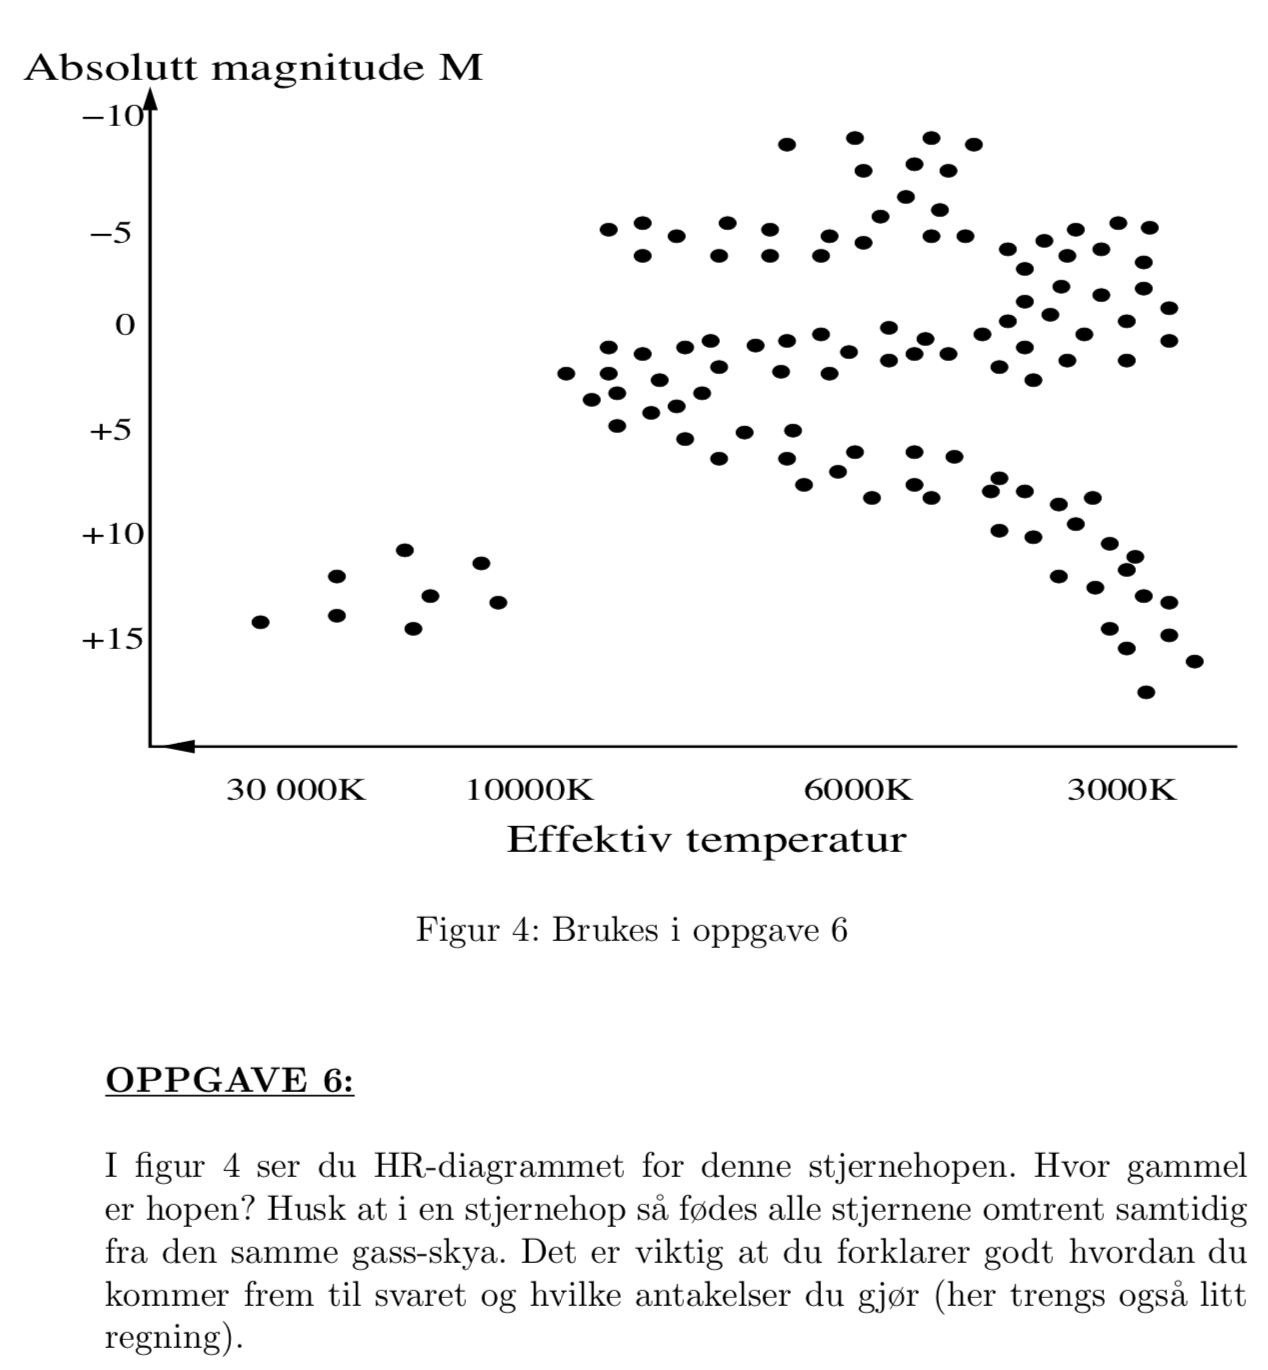
\includegraphics[scale=0.3]{media/eksamen_2011_oppg6.png}
}{SIDE 56/57/57}

\fullframetwo{se10}{se9}{oppsummering}{0}{\Large
Du trenger å kombinere nesten alt det du har lært i del 3D for å løse denne oppgaven. Når du har tenkt nøye gjennom hvordan denne oppgaven kan løses, og hvis du ikke ser det, ta en titt på \href{https://www.uio.no/studier/emner/matnat/astro/AST2000/h20/undervisningsmateriell/interaktive-forelesningsnotater/3d/videoer/video3d_6.mp4}{denne videoen}.
}
{\textcolor{red}{\bf Oppg.6, avsl. eksamen 2011:}
\hspace*{-0.4cm}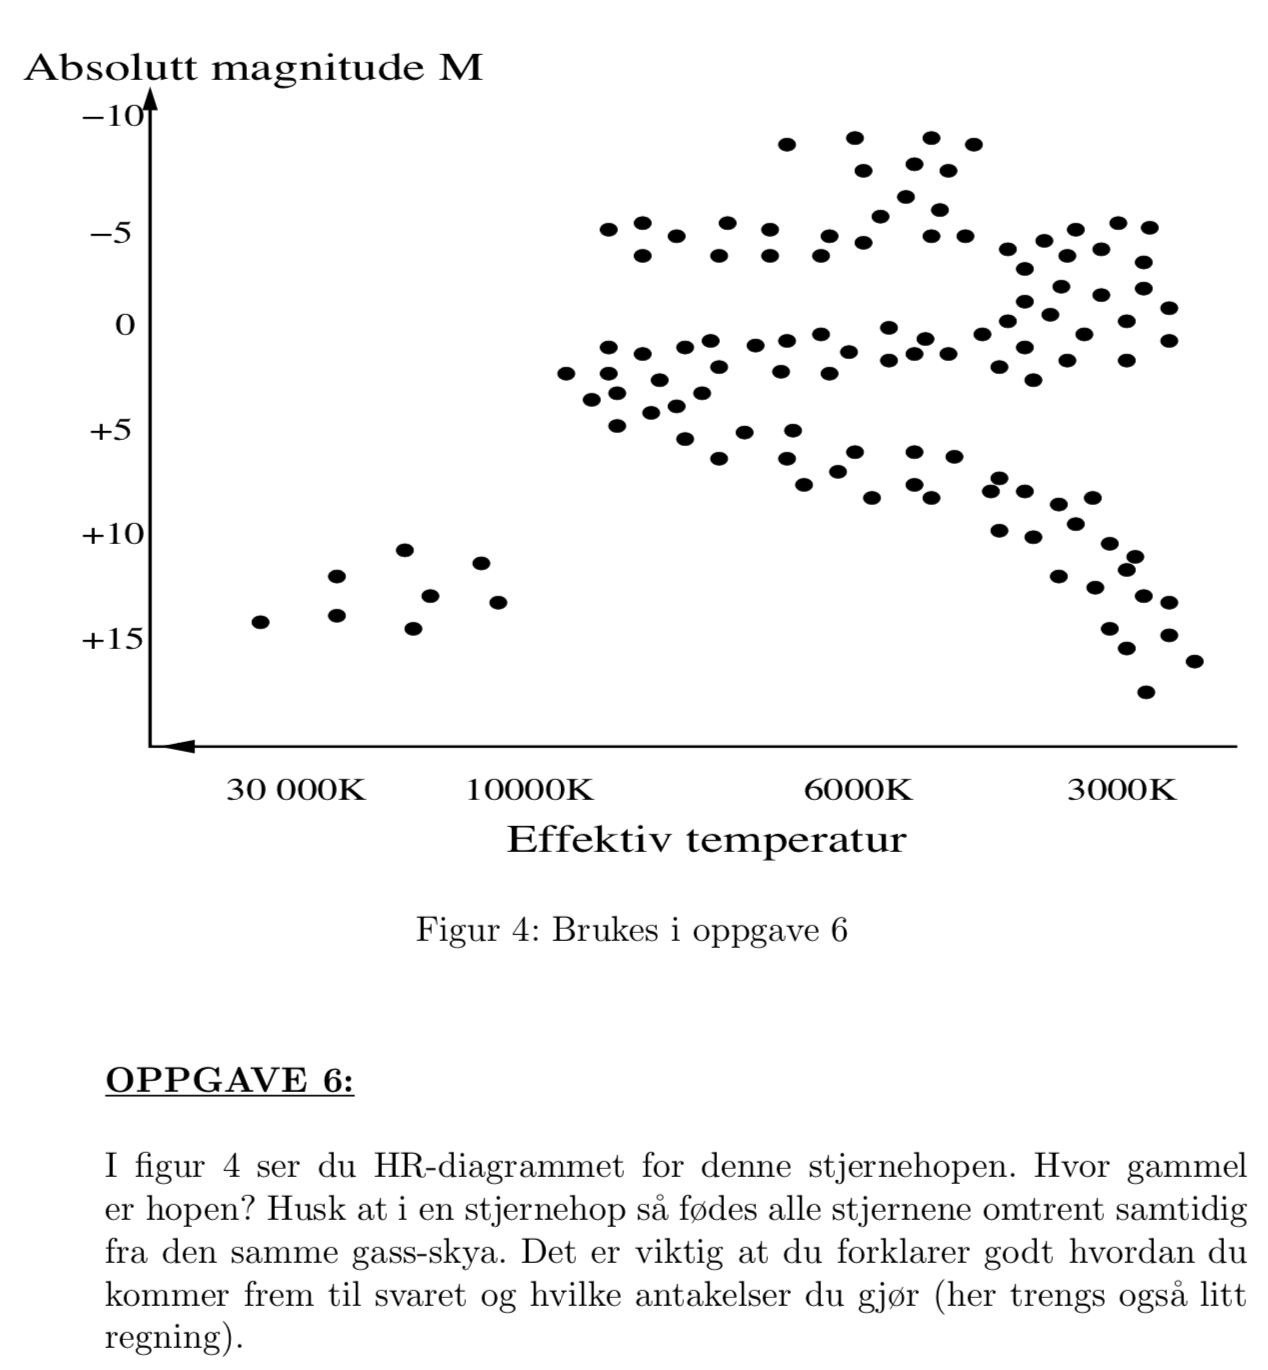
\includegraphics[scale=0.3]{media/eksamen_2011_oppg6.png}
}{SIDE 57/57/57}

\begin{frame}
\label{oppsummering}
\hyperlink{se10}{\pagebutton{\small Forrige side}}\href{https://nettskjema.no/a/167471}{\Changey[1][yellow]{2} \Changey[1][yellow]{-2}}
Gratulerer, del 3D er overstått. Du bør nå:
\begin{itemize}
\item  Vite hvilke størrelser og enheter man kan ha på aksene i et HR-diagram
\item  Vite hvorfor hovedserien er en skrå linje i HR-diagrammet
\item  Vite hvilke masser og radier stjerner kan ha og hvorfor
\item  Kunne gjøre overslagsregning med fysiske problemstillinger
\item  Kunne hovedtrekkene i hvordan vi finner tilnærmede sammenhenger mellom luminositet, levetid og overflatetemperatur på en stjerne og denne stjernens masse.
\item Kunne bruke proporsjonalitetsrelasjonene for stjerner
\item Kunne skissere de forskjellige overgangene som aldrende stjerner går gjennom på sin vei fra hovedserie til død, og kunne forstå årsakene til overgangene samt skissere og forklare hvordan de beveger seg i HR-diagrammet.
\end{itemize}
\textcolor{red}{Flott hvis du nå kan klikke på smilefjesene over og fortelle hva du synes om dette interaktive forelesningsnotatet. Hva var bra og nøyaktig hva kan forbedres? All ris og ros mottaes med takk!}
{\bf Det anbefales nå at du sjekker \href{https://www.uio.no/studier/emner/matnat/astro/AST2000/h21/undervisningsmateriell/kortsvarsoppgaver/del3d.pdf}{kortsvarsoppgavene} til del 3D for å kontrollere at du har forstått stoffet. Kan du svare på disse, blir det lettere å bruke kunnskapen din i oppgavene/prosjektet. Noen av disse kommer på eksamen.}
\end{frame}



\end{document}
